% RMS wrote:
%The text does not mention GNU anywhere.  This paper is an opportunity
%to make people aware of GNU, but the current text fails to use the
%opportunity.
%
%It should say that Taler is a GNU package.
%
%I suggest using the term "GNU Taler" in the title, once in the
%abstract, and the first time the name is mentioned in the body text.
%In the body text, it can have a footnote with more information
%including a reference to http://gnu.org/gnu/the-gnu-project.html.
%
%At the top of page 3, where it says "a free software implementation",
%it should add "(free as in freedom)", with a reference to
%http://gnu.org/philosophy/free-sw.html and
%http://gnu.org/philosophy/free-software-even-more-important.html.
%
%Would you please include these things in every article or posting?
%
% CG adds:
% We SHOULD do this for the FINAL paper, not for the anon submission.

\documentclass{llncs}
%\usepackage[margin=1in,a4paper]{geometry}
\usepackage[T1]{fontenc}
\usepackage{palatino}
\usepackage{xspace}
\usepackage{microtype}
\usepackage{tikz,eurosym}
\usepackage{amsmath,amssymb}
\usepackage{enumitem}
\usetikzlibrary{shapes,arrows}
\usetikzlibrary{positioning}
\usetikzlibrary{calc}

% Relate to:
% http://fc14.ifca.ai/papers/fc14_submission_124.pdf

% Terminology:
% - SEPA-transfer -- avoid 'SEPA transaction' as we use
%       'transaction' already when we talk about taxable
%        transfers of Taler coins and database 'transactions'.
% - wallet = coins at customer
% - reserve = currency entrusted to mint waiting for withdrawal
% - deposit = SEPA to mint
% - withdrawal = mint to customer
% - spending = customer to merchant
% - redeeming = merchant to mint (and then mint SEPA to merchant)
% - refreshing = customer-mint-customer
% - dirty coin = coin with exposed public key
% - fresh coin = coin that was refreshed or is new
% - coin signing key = mint's online key used to (blindly) sign coin
% - message signing key = mint's online key to sign mint messages
% - mint master key = mint's key used to sign other mint keys
% - owner = entity that knows coin private key
% - transaction = coin ownership transfer that should be taxed
% - sharing = coin copying that should not be taxed


\title{Taler: Taxable Anonymous Libre Electronic Reserves}

\begin{document}
\mainmatter

%\author{Florian Dold \and Sree Harsha Totakura \and Benedikt M\"uller \and Christian Grothoff}
%\institute{The GNUnet Project}


\maketitle

\begin{abstract}
This paper introduces Taler, a Chaum-style digital currency using
blind signatures that enables anonymous payments while ensuring that
entities that receive payments are auditable and thus taxable.  Taler
differs from Chaum's original proposal in that customers can never
defraud anyone, merchants can only fail to deliver the merchandise to
the customer, and mints can be fully audited. Consequently,
enforcement of honest behavior is better and more timely than with
Chaum, and is at least as strict as with legacy credit card payment
systems that do not provide for privacy.  Furthermore, Taler allows
fractional payments, and even in this case is still able to guarantee
unlinkability of transactions via a new coin refreshing protocol.  We
argue that Taler provides a secure digital currency for modern liberal
societies as it is a flexible, libre and efficient protocol and
adequately balances the state's need for monetary control with the
citizen's needs for private economic activity.
\end{abstract}

\section{Introduction}

The design of payment systems shapes economies and societies.  Strong,
developed nation states are evolving towards fully transparent payment
systems, such as the MasterCard and VisaCard credit card schemes and
computerized bank transactions such as SWIFT.  Such systems enable
mass surveillance and thus extensive government control over the
economy, from taxation to intrusion into private lives.  Bribery and
corruption are limited to elites that can afford to escape the
dragnet.  The other extreme are economies of developing, weak nation
states where economic activity is based largely on coins, paper money
or even barter.  Here, the state is often unable to effectively
monitor or tax economic activity, and this limits the ability of the
state to shape the society.  As bribery is virtually impossible to
detect, corruption is widespread and not limited to social elites.
ZeroCoin~\cite{miers2013zerocoin} is an example for translating such
an economy into the digital realm.

This paper describes Taler, a simple and practical payment system for
a modern social-liberal society, which is not being served well by
current payment systems which enable either an authoritarian state in
total control of the population, or create weak states with almost
anarchistic economies.

The Taler protocol is heavily based on ideas from
Chaum~\cite{chaum1983blind} and also follows Chaum's basic architecture of
customer, merchant and mint (Figure~\ref{fig:cmm}). The two designs
share the key first step where the {\em customer} withdraws digital
{\em coins} from the {\em mint} with unlinkability provided via blind
signatures.  The coins can then be spent at a {\em merchant} who {\em
  deposits} them at the mint.  Taler uses online detection of
double-spending, thus assuring the merchant instantly that a
transaction is valid.

\begin{figure}[h]
\centering
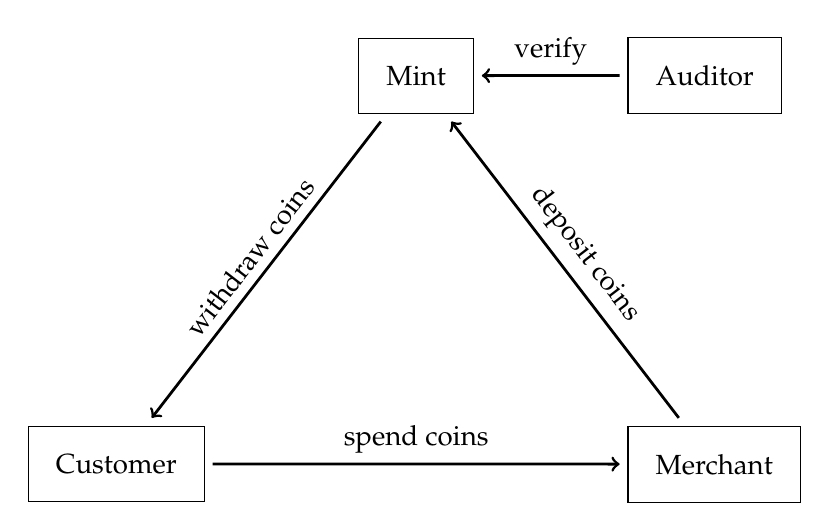
\begin{tikzpicture}
 \tikzstyle{def} = [node distance= 5em and 7em, inner sep=1em, outer sep=.3em];
 \node (origin) at (0,0) {};
 \node (mint) [def,above=of origin,draw]{Mint};
 \node (customer) [def, draw, below left=of origin] {Customer};
 \node (merchant) [def, draw, below right=of origin] {Merchant};
 \node (auditor) [def, draw, above right=of origin]{Auditor};

 \tikzstyle{C} = [color=black, line width=1pt]

 \draw [<-, C] (customer) -- (mint) node [midway, above, sloped] (TextNode) {withdraw coins};
 \draw [<-, C] (mint) -- (merchant) node [midway, above, sloped] (TextNode) {deposit coins};
 \draw [<-, C] (merchant) -- (customer) node [midway, above, sloped] (TextNode) {spend coins};
 \draw [<-, C] (mint) -- (auditor) node [midway, above, sloped] (TextNode) {verify};

\end{tikzpicture}
\caption{Taler's system model for the payment system is based on Chaum~\cite{chaum1983blind}.}
\label{fig:cmm}
\end{figure}

Taler was designed for use in a modern social-liberal society, which we
believe needs a payment system with the following properties:

\begin{description}
  \item[Customer Anonymity]
    It must be impossible for mints, merchants and even a global active
    adversary, to trace the spending behavior of a customer.
  \item[Unlinkability]
    As a strong form of customer anonymity, it must be infeasible to
    link a set of transactions to the same (anonymous) customer.
    %, even when taking aborted transactions into account.
  \item[Taxability]
    In many current legal systems, it is the responsibility of the merchant
    to deduct (sales) taxes from purchases made by customers, or to
    pay (income) taxes for payments received for work.
    %Taxation is necessary for the state to
    %provide legitimate social functions, such as education.  Thus, a payment
    %system must facilitate sales, income and transaction taxes.
    This requires that merchants are easily identifiable and that
    an audit trail is always generated, so that the state can ensure that its
    taxation regime is obeyed.
  \item[Verifiability]
    The payment system should try to minimize the trust necessary between
    the participants.  In particular, digital signatures should be used,
    and retained, whenever they would play a role in resolving disputes. % between the involved parties.
    Nevertheless, customers must never be able to defraud anyone, and
    merchants must at best be able to defraud their customers by not
    delivering on the agreed contract.  Neither merchants nor customers
    should ever be able to commit fraud against the mint.  Additionally,
    both customers and merchants must receive cryptographic proofs of
    bad behavior in case of protocol violations by the mint.
    In this way, only the mint will need to be tightly audited and regulated.
    The design must make it easy to audit the finances of the mint.
  \item[Ease of Deployment] %The system should be easy to deploy for
 %   real-world applications.  In order to lower the entry barrier and
 %   acceptance of the system, a gateway to the existing financial
 %   system should be provided, i.e. by integrating internet-banking
 %   protocols such as HBCI/FinTAN.
    The digital coins should be denominated in existing currencies,
    such as EUR or USD, to avoid exposing citizens to unnecessary risks
    from currency fluctuations.
    Moreover, the system must have an open protocol specification and
    a free software reference implementation.
%    The protocol should
%    be able to run easily over HTTP(S).
  \item[Low resource consumption]
    In order to minimize the operating costs and environmental impact of
    the payment system, it should avoid the reliance on expensive or
    ``wasteful'' computations, such as proof-of-work.
  \item[Fractional payments]
    The payment system needs to handle both small and large payments in
    an efficient and reliable manner.  It is inefficient to simply issue
    coins in the smallest unit of currency, so instead a mechanism to
    give {\em change} should be provided to ensure that customers with
    sufficient total funds can always spend them.
\end{description}
%
We give a concise example of how these properties interact:
A customer may want to pay \EUR{49,99} using a \EUR{100,00} coin.
the system must thus support giving change in the form of spendable coins,
say a \EUR{0,01} coin and a \EUR{50,00} coin.
A merchant cannot simply give the customer their coins in another transaction,
however, as this reverses the role of merchant and customer, and
our taxability requirement would deanonymize the customer.  The customer
also cannot withdraw exact change from his account from the mint, as this
would allow the mint to link the identity of the customer that is revealed
during withdrawal to the subsequent deposit operation that follows shortly
afterwards.
Instead, the customer should obtain new freshly anonymized coins that cannot be
linked with this transaction, the original \EUR{100,00} coin, or each other.

Instead of using cryptographic methods like $k$-show
signatures~\cite{brands1993efficient} to achieve divisibility,
Taler's fractional payments use a simpler, more powerful mechanism.
In Taler, a coin is not simply a signed unique random token, but signature
over the hash of a public key where the private key is only known to the owner
of the coin.
A customer transfers currency from a coin to a merchant by cryptographically
signing a deposit message with this private key.  This deposit message
specifies the fraction of the coin's value to be paid to the merchant.
A key contribution of Taler is the {\em refresh} protocol, which enables
a customer to exchange the residual value of the exchanged coin for
unlinkable fleshy anonymized change.

Taler mints ensure that all transactions involving the same coin
do not exceed the total value of the coin simply by
requiring that merchants clear transactions immediately with the mint.
This improves dramatically on systems that support offline merchants with
cryptographic threats to deanonymizing customers who double-spend, like
restrictive blind signatures~\cite{brands1993efficient}.
In such schemes, if a transaction is interrupted, then any coins sent to
the merchant become tainted, but may never arrive or be spent.
It becomes tricky to extract the value of the tainted coins without linking
to the aborted transaction and risking deanonymization.
As with support for fractional payments, Taler addresses these problems by
allowing customers to refresh tainted coins, thereby destroying the link
between the refunded or aborted transaction and the coin.

Taler ensures that the {\em entity} of the user owning the new coin is
the same as the entity of the user owning the old coin, thus making
sure that the refreshing protocol cannot be abused for money
laundering or other illicit transactions.


\section{Related Work}

\subsection{Blockchain-based currencies}

In recent years, a class of decentralized electronic payment systems,
based on collectively recorded and verified append-only public
ledgers, have gained immense popularity.  The most well-known protocol
in this class is Bitcoin~\cite{nakamoto2008bitcoin}.  An initial
concern with Bitcoin was the lack of anonymity, as all Bitcoin
transactions are recorded for eternity, which can enable
identification of users.  In theory, this concern has been addressed
with the Zerocoin extension to the protocol~\cite{miers2013zerocoin}.

These protocols do dispense with the need for a central, trusted
authority, while providing a useful measure of pseudonymity.
Yet, there are several major irredeemable problems inherent in their designs:

\begin{itemize}
  \item The computational puzzles solved by Bitcoin nodes with the purpose
    of securing the block chain consume a considerable amount of computational
    resources and energy.  So Bitcoin does not an environmentally responsible
    design.
  \item Bitcoin transactions are not easily taxable, leading to legal hurdles.
    % The legality and legitimacy of this aspect is questionable.
    The Zerocoin extension would only make this worse.
  \item Bitcoins can not easily be bound to any fiat currency, leading to
    significant fluctuations in value.  These fluctuations may be desirable in
    a high-risk investment instrument, but they make Bitcoin unsuitable as
    a medium of exchange.
  \item Worse, anyone can start an alternative Bitcoin transaction chain,
    called an AltCoin, and, if successful, reap the benefits of the low
    cost to initially create coins via computation.  As participants are
    de facto investors, these become a form of ponzi scheme.
    % As a result, dozens of
    % AltCoins have been created, often without any significant changes to the
    % technology.  A large number of AltCoins creates additional overheads for
    % currency exchange and exacerbates the problems with currency fluctuations.
\end{itemize}

GreenCoinX\footnote{\url{https://www.greencoinx.com/}} is a more
recent AltCoin where the company promises to identify the owner of
each coin via e-mail addresses and phone numbers.  While it is unclear
from their technical description how this identification would be
enforced against a determined adversary, the resulting payment system
would also merely impose a totalitarian financial panopticon on a
BitCoin-style money supply and transaction model, thus largely
combining what we would consider to be the drawbacks of these existing
systems.

\subsection{Chaum-style electronic cash}

Taler builds on ideas from Chaum~\cite{chaum1983blind}, who proposed a
digital payment system that would provide some customer anonymity
while disclosing the identity of the merchants.  Chaum's digital cash
system DigiCash had some limitations and ultimately failed to be widely
adopted.  In our assessment, key reasons for DigiCash's failure that
Taler avoids include:

\begin{itemize}
 \item The use of patents to protect the technology; a payment system
   should be free software (libre) to have a chance for widespread adoption.
 \item The use of off-line payments and thus deferred detection of
   double-spending, which could require the mint to attempt to recover
   funds from customers via the legal system.  This creates a
   significant business risk for the mint, as the system is not
   self-enforcing from the perspective of the mint.  In 1983 off-line
   payments might have been a necessary feature.  However, today
   requiring network connectivity is feasible and avoids the business
   risks associated with deferred fraud detection.
 \item % In addition to the risk of legal disputes with fraudulent
   % merchants and customers,
   Chaum's published design does not clearly
   limit the financial damage a mint might suffer from the
   disclosure of its private online signing key.
 \item Chaum did not support fractional payments or refunds without
   breaking customer anonymity.
%, and Brand's
%   extensions for fractional payments broke unlinkability and thus
%   limited anonymity.
% \item Chaum's system was implemented at a time where the US market
%   was still dominated by paper checks and the European market was
%   fragmented into dozens of currencies.  Today, SEPA provides a
%   unified currency and currency transfer method for most of Europe,
%   significantly lowering the barrier to entry into this domain for
%   a larger market.
\end{itemize}

Chaum's original digital cash system~\cite{chaum1983blind} was
extended by Brands~\cite{brands1993efficient} with the ability to {\em
  divide} coins and thus spend certain fractions of a coin using
restrictive blind signatures.  Compared to Taler, performing
fractional payments is cryptographically way more expensive and
moreover the transactions performed with ``divisions'' from the same
coin do become linkable.
%
%Some argue that the focus on technically perfect but overwhelmingly
%complex protocols, as well as the the lack of usable, practical
%solutions lead to an abandonment of these ideas by
%practitioners~\cite{selby2004analyzing}.
%

To our knowledge, the only publicly available effort to implement
Chaum's idea is Opencoin~\cite{dent2008extensions}.  However, Opencoin
seems to be neither actively developed nor used, and it is not clear
to what degree the implementation is even complete.  Only a partial
description of the Opencoin protocol is available to date.


\subsection{Peppercoin}

Peppercoin~\cite{rivest2004peppercoin} is a microdonation protocol.
The main idea of the protocol is to reduce transaction costs by
minimizing the number of transactions that are processed directly by
the mint.  Instead of always paying, the customer ``gambles'' with the
merchant for each microdonation.  Only if the merchant wins, the
microdonation is upgraded to a macropayment to be deposited at the
mint.  Peppercoin does not provide customer-anonymity.  The proposed
statistical method by which mints detect fraudulent cooperation between
customers and merchants at the expense of the mint not only creates
legal risks for the mint, but would also require that the mint learns
about microdonations where the merchant did not get upgraded to a
macropayment.  It is therefore unclear how Peppercoin would actually
reduce the computational burden on the mint.


\section{Design}

The payment system we propose is built on the blind signature
primitive proposed by Chaum, but extended with additional
constructions to provide unlinkability, online fraud detection and
taxability.

As with Chaum, the Taler system comprises three principal types of
actors (Figure~\ref{fig:cmm}): The \emph{customer} is interested in
receiving goods or services from the \emph{merchant} in exchange for
payment.  When making a transaction, both the customer and the
merchant must agree on the same \emph{mint}, which serves as an
intermediary for the financial transaction between the two.  The mint
is responsible for allowing the customer to obtain the anonymous
digital currency and for enabling the merchant to convert the
digital coins back to some traditional currency.  The \emph{auditor}
assures customers and merchants that the mint operates correctly.

\subsection{Security model}

Taler's security model assumes that cryptographic primitives are
secure and that each participant is under full control of his system.
The contact information of the mint is known to both customer and
merchant from the start.  Furthermore, the merchant communication's
authenticity is assured to the customer, such as by using X.509
certificates~\cite{rfc5280}, and we assume that an anonymous, reliable
bi-directional communication channel can be established by the
customer to both the mint and the merchant, such as by using Tor.

The mint is trusted to hold funds of its customers and to forward them
when receiving the respective deposit instructions from the merchants.
Customer and merchant can have some assurances about the mint's
liquidity and operation, as the mint has proven reserves, is subject
to the law, and can have its business regularly audited
 by a government or third party.
Regular audits of the mint's accounts should reveal any possible fraud
before the mint is allowed to destroy the corresponding accumulated
cryptographic proofs and book its fees as profits.
%
The merchant is trusted to deliver the service or goods to the
customer upon receiving payment.  The customer can seek legal relief
to achieve this, as he must get cryptographic proofs of the contract
and that he paid his obligations.
%
Neither the merchant nor the customer may have any ability to {\em
  effectively} defraud the mint or the state collecting taxes.  Here,
``effectively'' means that the expected return for fraud is negative.
Note that customers do not need to be trusted in any way, and that in
particular it is never necessary for anyone to try to recover funds
from customers using legal means.


\subsection{Taxability and Entities}

As electronic coins are trivially copied between machines, we should
clarify what kinds of operations can even be expected to be taxed.
After all, without intrusive measures to take away control of the
computing platform from its users, copying an electronic wallet from
one computer to another can hardly be prevented by a payment system.
Furthermore, it would also hardly be appropriate to tax the moving of
funds between two computers owned by the same entity.  We thus
need to clarify which kinds of transfers we expect to tax.

Taler is supposed to ensure that the state can tax {\em transactions}.
A {\em transaction} is a transfer where it is assured that one entity
gains control over funds while at the same time another entity looses
control over those funds.  We further restrict transactions to apply
only to the transfer of funds between {\em mutually distrustful}
entities.  Two entities are assumed to be mutually distrustful if they
are unwilling to share control over coins.  If a private key is shared
between two entities, then both entities have equal access to the
credentials represented by the private key.  In a payment system this
means that either entity could spent the associated funds.  Assuming
the payment system has effective double-spending detection, this means
that either entity has to constantly fear that the funds might no
longer be available to it.  It follows that sharing coins by copying
a private key implies mutual trust between the two parties, in which
case Taler will treat them as the same entity.
In Taler, making funds available by copying a private key and thus
sharing control is {\bf not} considered a {\em transaction} and
thus {\bf not} recorded for taxation.

Taler ensures taxability only when some entity acquires exclusive
control over the value of digital coins, which requires an interaction
with the mint.  For such transactions, the state can obtain information
from the mint, or a bank, that identifies the entity that received the
digital coins as well as the exact value of those coins.
Taler also allows the mint, and hence the state, to learn the value of
digital coins withdrawn by a customer---but not how, where, or when
they were spent.

\subsection{Anonymity}

An anonymous communication channel such as Tor~\cite{tor-design} is
used for all communication between the customer and the merchant.
Ideally, the customer's anonymity is limited only by this channel;
however, the payment system does additionally reveal that the customer
is one of the patrons of the mint.
There are naturally risks that the customer-merchant business operation
may leak identifying information about the customer.   At least, customers
have some options to defend their privacy against nosey merchants however,
possibly even when dealing with physical goods \cite{apod}.
We consider information leakage specific to the business logic to be
outside of the scope of the design of Taler.

Ideally, customer should use an anonymous communication channel with
the mint to avoid leaking IP address information; however, the mint
would typically learn the customer's identity from the wire transfer
that funds the customer's withdraw anonymous digital coins.
In fact, this is desirable as there might be rules and regulations
designed to limit the amount of anonymous digital cash that an
individual customer can withdraw in a given time period, similar to
how states today sometimes impose limits on cash
withdrawals~\cite{france2015cash,greece2015cash}.
Taler is only anonymous with respect to {\em payments}, as the mint
will be unable to link the known identity of the customer that withdrew
anonymous digital currency to the {\em purchase} performed later at the
merchant.  In this respect, Taler provides exactly the same scheme for
unconditional anonymous payments as was proposed by
Chaum~\cite{chaum1983blind,chaum1990untraceable} over 30 years ago.

While the customer thus has anonymity for purchases, the mint will
always learn the merchant's identity in order to credit the merchant's
account.  This is simply necessary for taxation, as Taler is supposed
to make information about funds received by any entity transparent
to the state.
% Technically, the merchant could still
%use an anonymous communication channel to communicate with the mint.
%However, in order to receive the traditional currency the mint will
%require (SEPA) account details for the deposit.

%As both the initial transaction between the customer and the mint as
%well as the transactions between the merchant and the mint do not have
%to be done anonymously, there might be a formal business contract
%between the customer and the mint and the merchant and the mint.  Such
%a contract may provide customers and merchants some assurance that
%they will actually receive the traditional currency from the mint
%given cryptographic proof about the validity of the transaction(s).
%However, given the business overheads for establishing such contracts
%and the natural goal for the mint to establish a reputation and to
%minimize cost, it is more likely that the mint will advertise its
%external auditors and proven reserves and thereby try to convince
%customers and merchants to trust it without a formal contract.


\subsection{Coins}

A \emph{coin} in Taler is a public-private key pair which derives its
financial value from a signature over the coin's public key by a mint.
The mint is expected to have multiple {\em coin signing key} pairs
available for signing, each representing a different coin
denomination.

These coin signing keys have an expiration date, before which any coins
signed with it must be spent or refreshed.  This allows the mint to
eventually discard records of old transactions, thus limiting the
records that the mint must retain and search to detect double-spending
attempts.  Furthermore, the mint is expected to use each coin signing
key only for a limited number of coins.
% for example by limiting its use to sign coins to a week or a month.
In this way, if a private coin signing key were to be compromised,
the mint would detect this once more coins were redeemed than the total
that was signed into existence using that coin signing key.
In this case, the mint could allow authentic customers to exchange their
unspent coins that were signed with the compromised private key,
while refusing further anonymous transactions involving those coins.
As a result, the financial damage of losing a private signing key can be
limited to at most twice the amount originally signed with that key.
To ensure that the mint does not enable deanonymization of users by
signing each coin with a fresh coin signing key, the mint must publicly
announce the coin signing keys in advance.  Those announcements are
expected to be signed with an off-line long-term private {\em master
signing key} of the mint and the auditor.

Before a customer can withdraw a coin from the mint,
he has to pay the mint the value of the coin, as well as processing fees.
This is done using other means of payments, such as wire transfers or
by having a personal {\em reserve} at the mint,
 which is equivalent to a bank account with a positive balance.
Taler assumes that the customer has a {\em withdrawal authorization key}
to identify himself as authorized to withdraw funds from the reserve.
By signing the withdrawal request messages using this withdrawal
authorization key, the customer can prove to the mint that he is the
individual authorized to withdraw anonymous digital coins from his reserve.
The mint will record the withdrawal messages with the reserve record as
proof that the anonymous digital coin was created for the correct
customer.  We note that the specifics of how the customer authenticates
to the mint are orthogonal to the rest of the system, and
 multiple methods can be supported.
%To put it differently, unlike
%modern cryptocurrencies like BitCoin, Taler's design simply
%acknowledges that primitive accumulation~\cite{engels1844} predates
%the system and that a secure method to authenticate owners exists.

After a coin is minted, the customer is the only entity that knows the
private key of the coin, making him the \emph{owner} of the coin.
The coin can be identified by the mint by its public key; however, due
to the use of blind signatures, the mint does not learn the public key
during the minting process.  Knowledge of the private key of the coin
enables the owner to spent the coin.  If the private key is shared
with others, they also become owners of the coin.

\subsection{Coin spending}

To spend a coin, the coin's owner needs to sign a {\em deposit
  request} specifying the amount, the merchant's account information
and a {\em business transaction-specific hash} using the coin's
private key.  A merchant can then transfer this permission of the
coin's owner to the mint to obtain the amount in traditional currency.
If the customer is cheating and the coin was already spent, the mint
provides cryptographic proof of the fraud to the merchant, who will
then refuse the transaction.  The mint is typically expected to
transfer the funds to the merchant using a wire transfer or by
crediting the merchant's individual account, depending on what is
appropriate to the domain of the traditional currency.

To allow exact payments without requiring the customer to keep a large
amount of ``change'' in stock and possibly perform thousands of
signatures for larger transactions, the payment systems allows partial
spending where just a fraction of a coin's total value is transferred.
Consequently, the mint the must not only store the identifiers of
spent coins, but also the fraction of the coin that has been spent.


\subsection{Refreshing Coins}

In this and other scenarios it is thus possible that a customer has
revealed the public key of a coin to a merchant, but not ultimately
signed over the full value of the coin.  If the customer then
continues to directly use the coin in other transactions, merchants
and the mint could link the various transactions as they all share the
same public key for the coin.

The owner of such a {\em dirty} coin might therefore want to exchange it
for a {\em fresh} coin to ensure unlinkability with future transactions.
% with the previous operation.
Even if a coin is not dirty, the owner of a coin may want to exchange it
if the respective coin signing key is about to expire.  All of these
operations are supported with the {\em coin refreshing protocol}, which
allows the owner of a coin to {\em melt} it for fresh coins of the same
value with a new public-private key pairs.  Refreshing does not use the
ordinary spending operation as the owner of a coin should not have to
pay taxes on this operation.  Because of this, the refreshing protocol
must assure that owner stays the same.
% After all, the coin refreshing protocol must not be usable for transactions, as
% transactions in Taler must be taxable.

% Meh, this paragraph sucks :
We therefore demand two main properties from the refresh protocol:
First, the mint must not be able to link the fresh coin's public key to
the public key of the dirty coin.  Second, the mint can ensure that the
owner of the dirty coin can determine the private key of the
fresh coin, thereby preventing the refresh protocol from being used to
construct a transaction.

%As with other operations, the refreshing protocol must also protect
%the mint from double-spending; similarly, the customer has to have
%cryptographic evidence if there is any misbehavior by the mint.
%Finally, the mint may choose to charge a transaction fee for
%refreshing by reducing the value of the generated fresh coins
%in relation to the value of the melted coins.
%
%Naturally, all such transaction fees should be clearly stated as part
%of the business contract offered by the mint to customers and
%merchants.


\section{Taler's Cryptographic Protocols}

% In this section, we describe the protocols for Taler in detail.

For the sake of brevity, we assume that a recipient of a signed
message always first checks that the signature is valid, even though
this is not explicitly stated below.  Also, whenever a signed message
is transmitted, it is assumed that the receiver is told the public key
(or knows it from the context) and that the signature contains
additional identification as to the purpose of the signature, making
it impossible to use a signature in a different context.

When the mint signs messages (not coins), an {\em online message
  signing key} of the mint is used.  The mint's long-term offline key
is used to certify both the coin signing keys as well as the online
message signing key of the mint.  The mint's long-term offline key is
assumed to be well-known to both customers and merchants, for example
because it is certified by the auditors.

As we are dealing with financial transactions, we explicitly describe
whenever entities need to safely commit data to persistent storage.
As long as those commitments persist, the protocol can be safely
resumed at any step.  Commitments to disk are cumulative, that is an
additional commitment does not erase the previously committed
information.  Keys and thus coins always have a well-known expiration
date; information committed to disk can be discarded after the
expiration date of the respective public key.  Customers can also
discard information once the respective coins have been fully spent,
and merchants may discard information once payments from the mint have
been received (assuming records are also no longer needed for tax
authorities).  The mint's bank transfers dealing in traditional
currency are expected to be recorded for tax authorities to ensure
taxability.

\subsection{Withdrawal}

Let $G$ be the generator of an elliptic curve.  To withdraw anonymous
digital coins, the customer performs the following interaction with
the mint:

\begin{enumerate}
  \item The customer identifies a mint with an auditor-approved
        coin signing public-private key pair $K := (K_s, K_p)$
        and randomly generates:
        \begin{itemize}
           \item withdrawal key $W := (w_s,W_p)$ with private key $w_s$ and public key $W_p$,
           \item coin key $C := (c_s,C_p)$ with private key $c_s$ and public key $C_p := c_s G$,
           \item blinding factor $b$, and commits $\langle W, C, b \rangle$ to disk.
        \end{itemize}
  \item The customer transfers an amount of money corresponding to (at least) $K_p$ to the mint, with $W_p$ in the subject line of the transaction.
  \item The mint receives the transaction and credits the $W_p$ reserve with the respective amount in its database.
  \item The customer sends $S_W(B_b(C_p))$ to the mint to request withdrawal of $C$; here, $B_b$ denotes Chaum-style blinding with blinding factor $b$.
  \item The mint checks if the same withdrawal request was issued before; in this case, it sends $S_{K}(B_b(C_p))$ to the customer.\footnote{Here $S_K$
        denotes a Chaum-style blind signature with private key $K_s$.}
        If this is a fresh withdrawal request, the mint performs the following transaction:
        \begin{enumerate}
           \item checks if the reserve $W_p$ has sufficient funds for a coin of value corresponding to $K_p$
           \item stores the withdrawal request and response $\langle S_W(B_b(C_p)), S_K(B_b(C_p)) \rangle$ in its database for future reference,
           \item deducts the amount corresponding to $K_p$ from the reserve,
        \end{enumerate}
        and then sends $S_{K}(B_b(C_p))$ to the customer.
        If the guards for the transaction fail, the mint sends a descriptive error back to the customer,
        with proof that it operated correctly (i.e. by showing the transaction history for the reserve).
  \item The customer computes (and verifies) the unblinded signature $S_K(C_p) = U_b(S_K(B_b(C_p)))$.
        The customer writes $\langle S_K(C_p), c_s \rangle$ to disk (effectively adding the coin to the
        local wallet) for future use.
\end{enumerate}
We note that the authorization to create and access a reserve using a
withdrawal key $W$ is just one way to establish that the customer is
authorized to withdraw funds.  If a mint has other ways to securely
authenticate customers and establish that they are authorized to
withdraw funds, those can also be used with Taler.


\subsection{Exact and partial spending}

A customer can spend coins at a merchant, under the condition that the
merchant trusts the specific mint that minted the coin.  Merchants are
identified by their key $M := (m_s, M_p)$ where the public key $M_p$
must be known to the customer a priori.

The following steps describe the protocol between customer, merchant and mint
for a transaction involving a coin $C := (c_s, C_p)$, which was previously signed
by a mint's denomination key $K$, i.e. the customer possesses
$\widetilde{C} := S_K(C_p)$:

\begin{enumerate}
\item\label{contract} Let $\vec{D} := D_1, \ldots, D_n$ be the list of
  mints accepted by the merchant where each $D_j$ is a mint's public
  key.  The merchant creates a digitally signed contract $\mathcal{A}
  := S_M(m, f, a, H(p, r), \vec{D})$ where $m$ is an identifier for this
  transaction, $a$ is data relevant to the contract indicating which services
  or goods the merchant will deliver to the customer, $f$ is the price of the offer,
  and $p$ is the merchant's payment information (e.g. his IBAN number) and $r$ is
  a random nonce.  The merchant commits $\langle \mathcal{A}
  \rangle$ to disk and sends $\mathcal{A}$ to the customer.
\item\label{deposit} The customer must possess or acquire a coin minted by a mint that is
  accepted by the merchant, i.e. $K$ should be publicly signed by some $D_j
  \in \{D_1, D_2, \ldots, D_n\}$, and has a value $\geq f$. (The customer
  can of course also use multiple coins where the total value adds up to
  the cost of the transaction and run the following steps for each of
  the coins. However, for simplicity of the exposition here we will
  assume that one coin is sufficient.)
%
  The customer then generates a \emph{deposit-permission} $\mathcal{D} :=
  S_c(\widetilde{C}, m, f, H(a), H(p,r), M_p)$
  and sends $\langle \mathcal{D}, D_j\rangle$ to the merchant,
  where $D_j$ is the mint which signed $K$.
\item The merchant gives $(\mathcal{D}, p, r)$ to the mint, revealing $p$
  only to the mint.

\item The mint validates $\mathcal{D}$ and checks for double spending.
  If the coin has been involved in previous transactions and the new
  one would exceed its remaining value, it sends an error
  with the records from the previous transactions back to the merchant.
%
  If double spending is not found, the mint commits $\langle \mathcal{D} \rangle$ to disk
  and notifies the merchant that the deposit operation was successful.

\item The merchant commits and forwards the notification from the mint to the
  customer, confirming the success (or failure) of the operation.
\end{enumerate}

If a transaction is aborted after Step~\ref{deposit},
subsequent transactions with the same coin could be linked to the coin,
but not directly to the coin's owner.  The same applies to partially
spent coins (where $f$ is smaller than the actual value of the coin).
To unlink subsequent transactions from a coin, the customer has to
execute the coin refreshing protocol with the mint.

%\begin{figure}[h]
%\centering
%\begin{tikzpicture}
%
%\tikzstyle{def} = [node distance= 1em, inner sep=.5em, outer sep=.3em];
%\node (origin) at (0,0) {};
%\node (offer) [def,below=of origin]{make offer (merchant $\rightarrow$ customer)};
%\node (A) [def,below=of offer]{permit lock (customer $\rightarrow$ merchant)};
%\node (B) [def,below=of A]{apply lock (merchant $\rightarrow$ mint)};
%\node (C) [def,below=of B]{confirm (or refuse) lock (mint $\rightarrow$ merchant)};
%\node (D) [def,below=of C]{sign contract (merchant $\rightarrow$ customer)};
%\node (E) [def,below=of D]{permit deposit (customer $\rightarrow$ merchant)};
%\node (F) [def,below=of E]{make deposit (merchant $\rightarrow$ mint)};
%\node (G) [def,below=of F]{transfer confirmation (mint $\rightarrow$ merchant)};
%
%\tikzstyle{C} = [color=black, line width=1pt]
%\draw [->,C](offer) -- (A);
%\draw [->,C](A) -- (B);
%\draw [->,C](B) -- (C);
%\draw [->,C](C) -- (D);
%\draw [->,C](D) -- (E);
%\draw [->,C](E) -- (F);
%\draw [->,C](F) -- (G);
%
%\draw [->,C, bend right, shorten <=2mm] (E.east)
%      to[out=-135,in=-45,distance=3.8cm] node[left] {aggregate} (D.east);
%\end{tikzpicture}
%\caption{Interactions between a customer, merchant and mint in the coin spending
%  protocol}
%\label{fig:spending_protocol_interactions}
%\end{figure}


\subsection{Refreshing} \label{sec:refreshing}

The following refreshing protocol is executed in order to melt a dirty
coin $C'$ of denomination $K$ to obtain a fresh coin $\widetilde{C}$
with the same denomination.  In practice, Taler uses a natural
extension where multiple fresh coins are generated a the same time to
enable giving precise change matching any amount.  In the
protocol, $\kappa \ge 3$ is a security parameter and $G$ is the
generator of the elliptic curve.

\begin{enumerate}
  \item For each $i = 1,\ldots,\kappa$, the customer randomly generates
    \begin{itemize}
      \item transfer key $T^{(i)} := \left(t^{(i)}_s,T^{(i)}_p\right)$ where $T^{(i)}_p := t^{(i)}_s G$,
      \item coin key pair \\ $C^{(i)} := \left(c_s^{(i)}, C_p^{(i)}\right)$ where $C^{(i)}_p := c^{(i)}_s G$,
      \item blinding factors $b^{(i)}$.
    \end{itemize}
    The customer then computes $E^{(i)} := E_{K_i}\left(c_s^{(i)}, b^{(i)}\right)$ where $K_i := H(c'_s T_p^{(i)})$. (The encryption key $K_i$ is
    computed by multiplying the private key $c'_s$ of the original coin with the point on the curve
    that represents the public key $T^{(i)}_p$ of the transfer key $T^{(i)}$. This is basically DH between coin and transfer key.),
    and commits $\langle C', \vec{T}, \vec{C}, \vec{b} \rangle$ to disk.
  \item The customer computes $B^{(i)} := B_{b^{(i)}}(C^{(i)}_p)$  for $i \in \{1,\ldots,\kappa\}$ and sends a commitment
    $S_{C'}(\vec{E}, \vec{B}, \vec{T_p}))$ to the mint.
  \item The mint generates a random\footnote{Auditing processes need to assure $\gamma$ is unpredictable until this time to
    prevent the mint from assisting tax evasion.} $\gamma$ with $1 \le \gamma \le \kappa$ and
    marks $C'_p$ as spent by committing
    $\langle C', \gamma, S_{C'}(\vec{E}, \vec{B}, \vec{T}) \rangle$ to disk.
  \item The mint sends $S_K(C'_p, \gamma)$ to the customer.\footnote{Instead of $K$, it is also
    possible to use any equivalent mint signing key known to the customer here, as $K$ merely
    serves as proof to the customer that the mint selected this particular $\gamma$.}
  \item The customer commits $\langle C', S_K(C'_p, \gamma) \rangle$ to disk.
  \item The customer computes $\mathfrak{R} := \left(t_s^{(i)}\right)_{i \ne \gamma}$
        and sends $S_{C'}(\mathfrak{R})$ to the mint.
  \item \label{step:refresh-ccheck} The mint checks whether $\mathfrak{R}$ is consistent with the commitments;
    specifically, it computes for $i \not= \gamma$:

    \vspace{-2ex}
    \begin{minipage}{5cm}
    \begin{align*}
      \overline{K}_i :&= H(t_s^{(i)} C_p'), \\
      (\overline{c}_s^{(i)}, \overline{b_i}) :&= D_{\overline{K}_i}(E^{(i)}), \\
     \overline{C^{(i)}_p} :&= \overline{c}_s^{(i)} G,
     \end{align*}
     \end{minipage}
    \begin{minipage}{5cm}
      \begin{align*}
       \overline{T_p^{(i)}} :&= t_s^{(i)} G, \\ \\
      \overline{B^{(i)}} :&= B_{\overline{b_i}}(\overline{C_p^{(i)}}),
      \end{align*}
    \end{minipage}

    and checks if $\overline{B^{(i)}} = B^{(i)}$
    and $\overline{T^{(i)}_p} = T^{(i)}_p$.


  \item \label{step:refresh-done} If the commitments were consistent,
    the mint sends the blind signature $\widetilde{C} :=
    S_{K}(B^{(\gamma)})$ to the customer.  Otherwise, the mint responds
    with an error indicating the location of the failure.
\end{enumerate}

%\subsection{N-to-M Refreshing}
%
%TODO: Explain, especially subtleties regarding session key / the spoofing attack that requires signature.

\subsection{Linking}

For a coin that was successfully refreshed, the mint responds to a
request $S_{C'}(\mathtt{link})$ with $(T^{(\gamma)}_p$, $E^{(\gamma)},
\widetilde{C})$.
%
This allows the owner of the melted coin to also obtain the private
key of the new coin, even if the refreshing protocol was illicitly
executed with the help of another party who generated $C_s$ and only
provided $\vec{C_p}$ and other required information to the old owner.
As a result, linking ensures that access to the new coins minted by
the refresh protocol is always {\em shared} with the owner of the
melted coins.  This makes it impossible to abuse the refresh protocol
for {\em transactions}.

The linking request is not expected to be used at all during ordinary
operation of Taler.  If the refresh protocol is used by Alice to
obtain change as designed, she already knows all of the information
and thus has little reason to request it via the linking protocol.
The fundamental reason why the mint must provide the link protocol is
simply to provide a threat: if Bob were to use the refresh protocol
for a transaction of funds from Alice to him, Alice may use a link
request to gain shared access to Bob's coins. Thus, this threat
prevents Alice and Bob from abusing the refresh protocol to evade
taxation on transactions. If Bob trusts Alice to not execute the link
protocol, then they can already conspire to evade taxation by simply
exchanging the original private coin keys.  This is permitted in our
taxation model as with such trust they are assumed to be the same
entity.

The auditor can anonymously check if the mint correctly implements the
link request, thus preventing the mint operator from legally disabling
this protocol component.  Without the link operation, Taler would
devolve into a payment system where both sides can be anonymous, and
thus no longer provide taxability.


\subsection{Error handling}

During operation, there are three main types of errors that are
expected.  First, in the case of faulty clients, the responding server
will generate an error message with detailed cryptographic proofs
demonstrating that the client was faulty, for example by providing
proof of double-spending or providing the previous commit and the
location of the missmatch in the case of the reveal step in the
refresh protocol.  It is also possible that the server may claim that
the client has been violating the protocol.  In these cases, the
clients should verify any proofs provided and if they are acceptable,
notify the user that they are somehow faulty.  Similar, if the
server indicates that the client is violating the protocol, the
client should record the interaction and enable the user to file a
bug report.

The second case is a faulty mint service provider.  Such faults will
be detected because of protocol violations (for example, by providing
a faulty proof or no proof).  In this case, the client is expected to
notify the auditor, providing a transcript of the interaction.  The
auditor can then (anonymously) replay the transaction, and either
provide the (now) correct response to the client or take appropriate
legal action against the faulty provider.

The third case are transient failures, such as network failures or
temporary hardware failures at the mint service provider.  Here, the
client may receive an explicit protocol indication (such as an HTTP
response code 500 ``internal server error'') or simply no response.
The appropriate behavior for the client is to automatically retry
(after 1s, twice more at randomized times within 1 minute). If those
three attempts fail, the user should be informed about the delay.  The
client should then retry another three times within the next 24h, and
after that time the auditor be informed about the outage.

Using this process, short term failures should be effectively obscured
from the user, while malicious behavior is reported to the auditor who
can then presumably rectify the situation, for example by shutting
down the operator (while providing an opportunity for customers to
receive refunds for the coins in circulation).  To ensure that such
refunds are possible, the operator is expected to always provide
adequate securities for the amount of coins in circulation as part of
the certification process.

\subsection{Refunds}

The refresh protocol offers an easy way to enable refunds to
customers, even if they are anonymous.  Refunds can be supported
by including a public signing key of the merchant in the transaction
details, and having the customer keep the private key of the spent
coins on file.

Given this, the merchant can simply sign a {\em refund confirmation}
and share it with the mint (and the customer).  Assuming the mint has
a way to recover the funds from the merchant (or simply not performed
the wire transfer yet), the mint can simply add the value of the
refunded transaction back to the original coin, re-enabling those
funds to be spent again by the original customer.

The (anonymous) customer -- but nobody else -- can then use the
refresh protocol to melt the refunded coin and create a fresh coin
that is unlinkable to the refunded transaction.


\section{Discussion}

Taler's security is largely equivalent to that of Chaum's original
design without online checks (and without the cut-and-choose
revelation of double-spending customers for offline spending).  We
specifically note that the digital equivalent of the ``Columbian Black
Market Exchange''~\cite{fatf1997} is a theoretical problem for both
Chaum and Taler, as individuals with a strong mutual trust foundation
can simply copy electronic coins and thereby establish a limited form
of black transfers.  However, unlike the situation with physical
checks with blank recipients in the Columbian black market, the
transitivity is limited as each participant can deposit the electronic
coins and thereby cheat any other participant, while in the Columbian
black market each participant only needs to trust the issuer of the
check and not also all previous owners of the physical check.

As with any unconditionally anonymous payment system, the ``Perfect
Crime'' attack~\cite{solms1992perfect} where blackmail is used to
force the mint to issue anonymous coins also continues to apply in
principle.  However, as mentioned Taler does facilitate limits on
withdrawals, which we believe is a better trade-off than the
problematic escrow systems where the necessary intransparency
actually facilitates voluntary cooperation between the mint and
criminals~\cite{sander1999escrow} and where state can selectively
deanonymize activists to support the deep state's quest for absolute
security.

\subsection{Offline Payments}

Chaum's original proposals for anonymous digital cash avoided the need
for online interactions with the mint to detect double spending by
providing a means to deanonymize customers involved in
double-spending.  We believe that this is problematic as the mint or
the merchant will then still need out-of-band means to recover funds
from the customer, which may be impossible in practice.  In contrast,
in our design only the mint may try to defraud the other participants
and disappear.  While this is still a risk, and regular financial
audits are required to protect against it, this is more manageable and
significantly cheaper compared to recovering funds via the court
system from customers.

Chaum's method for offline payments would also be incompatible with
the refreshing protocol (Section~\ref{sec:refreshing}) which enables
the crucial feature of giving unlinkable change.  The reason is that
if the owner's identity were embedded in coins, it would be leaked to
the mint as part of the reveal operation in the cut-and-choose
operation of the refreshing protocol.

%\subsection{Merchant Tax Audits}
%
%For a tax audit on the merchant, the mint includes the business
%transaction-specific hash in the transfer of the traditional
%currency.  A tax auditor can then request the merchant to reveal
%(meaningful) details about the business transaction ($\mathcal{D}$,
%$a$, $p$, $r$), including proof that applicable taxes were paid.
%
%If a merchant is not able to provide theses values, he can be
%subjected to financial penalties by the state in relation to the
%amount transferred by the traditional currency transfer.

\subsection{Cryptographic proof vs. evidence}

In this paper we have use the term ``proof'' in many places as the
protocol provides cryptographic proofs of which parties behave
correctly or incorrectly. However, as~\cite{fc2014murdoch} point out,
in practice financial systems need to provide evidence that holds up
in courts.  Taler's implementation is designed to export evidence and
upholds the core principles described in~\cite{fc2014murdoch}.  In
particular, in providing the cryptographic proofs as evidence none of
the participants have to disclose their core secrets, the process is
covered by standard testing procedures, and the full trusted
computing base (TCB) is public and free software.

%\subsection{System Performance}
%
%We performed some initial performance measurements for the various
%operations on our mint implementation.  The main conclusion was that
%the computational and bandwidth cost for transactions described in
%this paper is smaller than $10^{-3}$ cent/transaction, and thus
%dwarfed by the other business costs for the mint.  However, this
%figure excludes the cost of currency transfers using traditional
%banking, which a mint operator would ultimately have to interact with.
%Here, mint operators should be able to reduce their expenses by
%aggregating multiple transfers to the same merchant.


%\section{Conclusion}

%We have presented an efficient electronic payment system that
%simultaneously addresses the conflicting objectives created by the
%citizen's need for privacy and the state's need for taxation.  The
%coin refreshing protocol makes the design flexible and enables a
%variety of payment methods.  The current balance and profits of the
%mint are also easily determined, thus audits can be used to ensure
%that the mint operates correctly.  The libre implementation and open
%protocol may finally enable modern society to upgrade to proper
%electronic wallets with efficient, secure and privacy-preserving
%transactions.

% commented out for anonymized submission
%\subsection*{Acknowledgements}

%This work was supported by a grant from the Renewable Freedom Foundation.
% FIXME: ARED?
%We thank Tanja Lange, Dan Bernstein, Luis Ressel and Fabian Kirsch for feedback on an earlier
%version of this paper, Nicolas Fournier for implementing and running
%some performance benchmarks, and Richard Stallman, Hellekin Wolf,
%Jacob Appelbaum for productive discussions and support.


\bibliographystyle{alpha}
\bibliography{taler,rfc}

\newpage
\appendix

\section{Optional features}

In this appendix we detail various optional features that can
be added to the basic protocol to reduce transaction costs for
certain interactions.

However, we note that Taler's transaction costs are expected to be so
low that these features are likely not particularly useful in
practice: When we performed some initial performance measurements for
the various operations on our mint implementation, the main conclusion
was that the computational and bandwidth cost for transactions
described in this paper is smaller than $10^{-3}$ cent/transaction,
and thus dwarfed by the other business costs for the mint.  We note
that the $10^{-3}$ cent/transaction estimate excludes the cost of wire
transfers using traditional banking, which a mint operator would
ultimately have to interact with.  Here, mint operators should be able
to reduce their expenses by aggregating multiple transfers to the same
merchant.

As a result of the low cost of the interaction with the mint in Taler
today, we expect that transactions with amounts below Taler's internal
transaction costs to be economically meaningless.  Nevertheless, we
document various ways how such transactions could be achieved within
Taler.



\subsection{Incremental spending}

For services that include pay-as-you-go billing, customers can over
time sign deposit permissions for an increasing fraction of the value
of a coin to be paid to a particular merchant.  As checking with the
mint for each increment might be expensive, the coin's owner can
instead sign a {\em lock permission}, which allows the merchant to get
an exclusive right to redeem deposit permissions for the coin for a
limited duration.  The merchant uses the lock permission to determine
if the coin has already been spent and to ensure that it cannot be
spent by another merchant for the {\em duration} of the lock as
specified in the lock permission.  If the coin has insufficient funds
because too much has been spent or is
already locked, the mint provides the owner's deposit or locking
request and signature to prove the attempted fraud by the customer.
Otherwise, the mint locks the coin for the expected duration of the
transaction (and remembers the lock permission).  The merchant and the
customer can then finalize the business transaction, possibly
exchanging a series of incremental payment permissions for services.
Finally, the merchant then redeems the coin at the mint before the
lock permission expires to ensure that no other merchant redeems the
coin first.

\begin{enumerate}
\item\label{offer2} The merchant sends an \emph{offer:} $\langle S_M(m, f),
  \vec{D} \rangle$ containing the price of the offer $f$, a transaction
  ID $m$ and the list of mints $D_1, \ldots, D_n$ accepted by the merchant
  where each $D_j$ is a mint's public key.
\item\label{lock2} The customer must possess or acquire a coin $\widetilde{C}$
  signed by a mint that is
  accepted by the merchant, i.e. $K$ should be signed by some $D_j
  \in \{D_1, D_2, \ldots, D_n\}$, and has a value $\geq f$.

  Customer then generates a \emph{lock-permission} $\mathcal{L} :=
  S_c(\widetilde{C}, t, m, f, M_p)$ where $t$ specifies the time until which the
  lock is valid and sends $\langle \mathcal{L}, D_j\rangle$ to the merchant,
  where $D_j$ is the mint which signed $K$.
\item The merchant asks the mint to apply the lock by sending $\langle
  \mathcal{L} \rangle$ to the mint.
\item The mint validates $\widetilde{C}$ and detects double spending
  in the form of existing \emph{deposit-permission} or
  lock-permission records for $\widetilde{C}$.  If such records exist
  and indicate that insufficient funds are left, the mint sends those
  records to the merchant, who can then use the records to prove the double
  spending to the customer.

  If double spending is not found,
  the mint commits $\langle \mathcal{L} \rangle$ to disk
  and notifies the merchant that locking was successful.
\item\label{contract2} The merchant creates a digitally signed contract
  $\mathcal{A} := S_M(m, f, a, H(p, r))$ where $a$ is data relevant to the contract
  indicating which services or goods the merchant will deliver to the customer, and $p$ is the
  merchant's payment information (e.g. his IBAN number) and $r$ is an random nonce.
  The merchant commits $\langle \mathcal{A} \rangle$ to disk and sends it to the customer.
\item The customer creates a
  \emph{deposit-permission} $\mathcal{D} := S_c(\widetilde{C}, \widetilde{L}, f, m, M_p, H(a), H(p, r))$, commits
  $\langle \mathcal{A}, \mathcal{D} \rangle$ to disk and sends $\mathcal{D}$ to the merchant.
\item\label{invoice_paid2} The merchant commits the received $\langle \mathcal{D} \rangle$ to disk.
\item The merchant gives $(\mathcal{D}, p, r)$ to the mint, revealing his
  payment information.
\item The mint verifies $(\mathcal{D}, p, r)$ for its validity and
  checks against double spending, while of
  course permitting the merchant to withdraw funds from the amount that
  had been locked for this merchant.
 \item If $\widetilde{C}$ is valid and no equivalent \emph{deposit-permission} for $\widetilde{C}$ and $\widetilde{L}$ exists on disk, the
  mint performs the following transaction:
  \begin{enumerate}
    \item $\langle \mathcal{D}, p, r \rangle$ is committed to disk.
    \item\label{transfer2} transfers an amount of $f$ to the merchant's bank account
      given in $p$.  The subject line of the transaction to $p$ must contain
      $H(\mathcal{D})$.
  \end{enumerate}
  Finally, the mint sends a confirmation to the merchant.
 \item If the deposit record $\langle \mathcal{D}, p, r \rangle$ already exists,
  the mint sends the confirmation to the merchant,
  but does not transfer money to $p$ again.
\end{enumerate}

To facilitate incremental spending of a coin $C$ in a single transaction, the
merchant makes an offer in Step~\ref{offer2} with a maximum amount $f_{max}$ he
is willing to charge in this transaction from the coin $C$.  After obtaining the
lock on $C$ for $f_{max}$, the merchant makes a contract in Step~\ref{contract2}
with an amount $f \leq f_{max}$.  The protocol follows with the following steps
repeated after Step~\ref{invoice_paid2} whenever the merchant wants to charge an
incremental amount up to $f_{max}$:

\begin{enumerate}
  \setcounter{enumi}{4}
\item The merchant generates a new contract $ \mathcal{A}' := S_M(m, f', a', H(p,
  r)) $ after obtaining the deposit-permission for a previous contract.  Here
  $f'$ is the accumulated sum the merchant is charging the customer, of which
  the merchant has received a deposit-permission for $f$ from the previous
  contract \textit{i.e.}~$f <f' \leq f_{max}$.  Similarly $a'$ is the new
  contract data appended to older contract data $a$.
  The merchant commits $\langle \mathcal{A}' \rangle$ to disk and sends it to the customer.
\item Customer commits $\langle \mathcal{A}' \rangle$ to disk, creates
  $\mathcal{D}' := S_c(\widetilde{C}, \mathcal{L}, f', m, M_p, H(a'), H(p, r))$, commits
  $\langle \mathcal{D'} \rangle$ and sends it to the merchant.
\item The merchant commits the received $\langle \mathcal{D'} \rangle$ and
  deletes the older $\mathcal{D}$.
\end{enumerate}

%Figure~\ref{fig:spending_protocol_interactions} summarizes the interactions of the
%coin spending protocol.

For transactions with multiple coins, the steps of the protocol are
executed in parallel for each coin.  During the time a coin is locked,
the locked fraction may not be spent at a different merchant or via a
deposit permission that does not contain $\mathcal{L}$.  The mint will
release the locks when they expire or are used in a deposit operation.
Thus the coins can be used with other merchants once their locks
expire, even if the original merchant never executed any deposit for
the coin.  However, doing so may link the new transaction to older
transaction.

Similarly, if a transaction is aborted after Step 2, subsequent
transactions with the same coin can be linked to the coin, but not
directly to the coin's owner.  The same applies to partially spent
coins.  Thus, to unlink subsequent transactions from a coin, the
customer has to execute the coin refreshing protocol with the mint.

%\begin{figure}[h]
%\centering
%\begin{tikzpicture}
%
%\tikzstyle{def} = [node distance= 1em, inner sep=.5em, outer sep=.3em];
%\node (origin) at (0,0) {};
%\node (offer) [def,below=of origin]{make offer (merchant $\rightarrow$ customer)};
%\node (A) [def,below=of offer]{permit lock (customer $\rightarrow$ merchant)};
%\node (B) [def,below=of A]{apply lock (merchant $\rightarrow$ mint)};
%\node (C) [def,below=of B]{confirm (or refuse) lock (mint $\rightarrow$ merchant)};
%\node (D) [def,below=of C]{sign contract (merchant $\rightarrow$ customer)};
%\node (E) [def,below=of D]{permit deposit (customer $\rightarrow$ merchant)};
%\node (F) [def,below=of E]{make deposit (merchant $\rightarrow$ mint)};
%\node (G) [def,below=of F]{transfer confirmation (mint $\rightarrow$ merchant)};
%
%\tikzstyle{C} = [color=black, line width=1pt]
%\draw [->,C](offer) -- (A);
%\draw [->,C](A) -- (B);
%\draw [->,C](B) -- (C);
%\draw [->,C](C) -- (D);
%\draw [->,C](D) -- (E);
%\draw [->,C](E) -- (F);
%\draw [->,C](F) -- (G);
%
%\draw [->,C, bend right, shorten <=2mm] (E.east)
%      to[out=-135,in=-45,distance=3.8cm] node[left] {aggregate} (D.east);
%\end{tikzpicture}
%\caption{Interactions between a customer, merchant and mint in the coin spending
%  protocol}
%\label{fig:spending_protocol_interactions}
%\end{figure}


\subsection{Probabilistic donations}

Similar to Peppercoin, Taler supports probabilistic {\em micro}donations of coins to
support cost-effective transactions for small amounts.  We consider
amounts to be ``micro'' if the value of the transaction is close or
even below the business cost of an individual transaction to the mint.

To support microdonations, an ordinary transaction is performed based
on the result of a biased coin flip with a probability related to the
desired transaction amount in relation to the value of the coin.  More
specifically, a microdonation of value $\epsilon$ is upgraded to a
macropayment of value $m$ with a probability of $\frac{\epsilon}{m}$.
Here, $m$ is chosen such that the business transaction cost at the
mint is small in relation to $m$.  The mint is only involved in the
tiny fraction of transactions that are upgraded.  On average both
customers and merchants end up paying (or receiving) the expected
amount $\epsilon$ per microdonation.

Unlike Peppercoin, in Taler either the merchant wins and the customer
looses the coin, or the merchant looses and the customer keeps the
coin.  Thus, there is no opportunity for the merchant and the customer
to conspire against the mint.  To determine if the coin is to be
transferred, merchant and customer execute a secure coin flipping
protocol~\cite{blum1981}.  The commit values are included in the
business contract and are revealed after the contract has been signed
using the private key of the coin.  If the coin flip is decided in
favor of the merchant, the merchant can redeem the coin at the mint.

One issue in this protocol is that the customer may use a worthless
coin by offering a coin that has already been spent.  This kind of
fraud would only be detected if the customer actually lost the coin
flip, and at this point the merchant might not be able to recover from
the loss.  A fraudulent anonymous customer may run the protocol using
already spent coins until the coin flip is in his favor.

As with incremental spending, lock permissions could be used to ensure
that the customer cannot defraud the merchant by offering a coin that
has already been spent.  However, as this means involving the mint
even if the merchant looses the coin flip, such a scheme is unsuitable
for microdonations as the transaction costs from involving the mint
might be disproportionate to the value of the transaction, and thus
with locking the probabilistic scheme has no advantage over simply
using fractional payments.

Hence, Taler uses probabilistic transactions {\em without} online
double-spending detection.  This enables the customer to defraud the
merchant by paying with a coin that was already spent.  However, as,
by definition, such microdonations are for tiny amounts, the incentive
for customers to pursue this kind of fraud is limited.  Still, to
clarify that the customer must be honest, we prefer the term
micro{\em donations} over micro{\em payments} for this scheme.


The following steps are executed for microdonations with upgrade probability $p$:
\begin{enumerate}
  \item The merchant sends an offer to the customer.
  \item The customer sends a commitment $H(r_c)$ to a random
    value $r_c \in [0,2^R)$, where $R$ is a system parameter.
  \item The merchant sends random $r_m \in [0,2^R)$ to the customer.
    \item The customer computes $p' := (|r_c - r_m|) / (2^R)$.
    If $p' < p$, the customer sends a coin with deposit-permission to the merchant.
    Otherwise, the customer sends $r_c$ to the merchant.
  \item The merchant deposits the coin, or checks if $r_c$ is consistent
    with $H(r_c)$.
\end{enumerate}

Evidently the customer can ``cheat'' by aborting the transaction in
Step 3 of the microdonation protocol if the outcome is unfavorable ---
and repeat until he wins.  This is why Taler is suitable for
microdonations --- where the customer voluntarily contributes ---
and not for micropayments.

Naturally, if the donations requested are small, the incentive to
cheat for minimal gain should be quite low.  Payment software could
embrace this fact by providing an appeal to conscience in form of an
option labeled ``I am unethical and want to cheat'', which executes
the dishonest version of the payment protocol.

If an organization detects that it cannot support itself with
microdonations, it can always choose to switch to the macropayment
system with slightly higher transaction costs to remain in business.

\newpage
\section{Notation summary}

The paper uses the subscript $p$ to indicate public keys and $s$ to
indicate secret (private) keys.  For keys, we also use small letters
for scalars and capital letters for points on an elliptic curve.  The
capital letter without the subscript $p$ stands for the key pair.  The
superscript $(i)$ is used to indicate one of the elements of a vector
during the cut-and-choose protocol.  Bold-face is used to indicate a
vector over these elements.  A line above indicates a value computed
by the verifier during the cut-and-choose operation.  We use $f()$ to
indicate the application of a function $f$ to one or more arguments.

\begin{description}
  \item[$K_s$]{Private (RSA) key of the mint used for coin signing}
  \item[$K_p$]{Public (RSA) key corresponding to $K_s$}
  \item[$K$]{Public-priate (RSA) coin signing key pair $K := (K_s, K_p)$}
  \item[$b$]{RSA blinding factor for RSA-style blind signatures}
  \item[$B_b()$]{RSA blinding over the argument using blinding factor $b$}
  \item[$U_b()$]{RSA unblinding of the argument using blinding factor $b$}
  \item[$S_K()$]{Chaum-style RSA signature, $S_K(C) = U_b(S_K(B_b(C)))$}
  \item[$w_s$]{Private key from customer for authentication}
  \item[$W_p$]{Public key corresponding to $w_s$}
  \item[$W$]{Public-private customer authentication key pair $W := (w_s, W_p)$}
  \item[$S_W()$]{Signature over the argument(s) involving key $W$}
  \item[$m_s$]{Private key from merchant for authentication}
  \item[$M_p$]{Public key corresponding to $m_s$}
  \item[$M$]{Public-private merchant authentication key pair $M := (m_s, M_p)$}
  \item[$S_M()$]{Signature over the argument(s) involving key $M$}
  \item[$G$]{Generator of the elliptic curve}
  \item[$c_s$]{Secret key corresponding to a coin, scalar on a curve}
  \item[$C_p$]{Public key corresponding to $c_s$, point on a curve}
  \item[$C$]{Public-private coin key pair $C := (c_s, C_p)$}
  \item[$S_{C}()$]{Signature over the argument(s) involving key $C$ (using EdDSA)}
  \item[$c_s'$]{Private key of a ``dirty'' coin (otherwise like $c_s$)}
  \item[$C_p'$]{Public key of a ``dirty'' coin (otherwise like $C_p$)}
  \item[$C'$]{Dirty coin (otherwise like $C$)}
  \item[$\widetilde{C}$]{Mint signature $S_K(C_p)$ indicating validity of a fresh coin (with key $C$)}
  \item[$n$]{Number of mints accepted by a merchant}
  \item[$j$]{Index into a set of accepted mints, $i \in \{1,\ldots,n\}$}
  \item[$D_j$]{Public key of a mint (not used to sign coins)}
  \item[$\vec{D}$]{Vector of $D_j$ signifying mints accepted by a merchant}
  \item[$a$]{Complete text of a contract between customer and merchant}
  \item[$f$]{Amount a customer agrees to pay to a merchant for a contract}
  \item[$m$]{Unique transaction identifier chosen by the merchant}
  \item[$H()$]{Hash function}
  \item[$p$]{Payment details of a merchant (i.e. wire transfer details for a bank transfer)}
  \item[$r$]{Random nonce}
  \item[${\cal A}$]{Complete contract signed by the merchant}
  \item[${\cal D}$]{Deposit permission, signing over a certain amount of coin to the merchant as payment and to signify acceptance of a particular contract}
  \item[$\kappa$]{Security parameter $\ge 3$}
  \item[$i$]{Index over cut-and-choose set, $i \in \{1,\ldots,\kappa\}$}
  \item[$\gamma$]{Selected index in cut-and-choose protocol, $\gamma \in \{1,\ldots,\kappa\}$}
  \item[$t^{(i)}_s$]{private transfer key, a scalar}
  \item[$T^{(i)}_s$]{private transfer key, point on a curve (same curve must be used for $C_p$)}
  \item[$T^{(i)}$]{public-private transfer key pair $T^{(i)} := (t^{(i)}_s,T^{(i)}_s)$}
  \item[$\vec{T}$]{Vector of $T^{(i)}$}
  \item[$c_s^{(i)}$]{Secret key corresponding to a fresh coin, scalar on a curve}
  \item[$C_p^{(i)}$]{Public key corresponding to $c_s^{(i)}$, point on a curve}
  \item[$C^{(i)}$]{Public-private coin key pair $C^{(i)} := (c_s^{(i)}, C_p^{(i)})$}
  \item[$\vec{C}$]{Vector of $C^{(i)}$ (public and private keys)}
  \item[$b^{(i)}$]{Blinding factor for RSA-style blind signatures}
  \item[$\vec{b}$]{Vector of $b^{(i)}$}
  \item[$B^(i)$]{Blinding of $C_p^{(i)}$}
  \item[$\vec{B}$]{Vector of $B^{(i)}$}
  \item[$K_i$]{Symmetric encryption key derived from ECDH operation via hashing}
  \item[$E_{K_i}()$]{Symmetric encryption using key $K_i$}
  \item[$E^{(i)}$]{$i$-th encryption of the private information $(c_s^{(i)}, b_i)$}
  \item[$\vec{E}$]{Vector of $E^{(i)}$}
  \item[$\cal{R}$]{Tuple of revealed vectors in cut-and-choose protocol,
    where the vectors exclude the selected index $\gamma$}
  \item[$\overline{K_i}$]{Encryption keys derived by the verifier from DH}
  \item[$\overline{B^{(i)}}$]{Blinded values derived by the verifier}
  \item[$\overline{T_p^{(i)}}$]{Public transfer keys derived by the verifier from revealed private keys}
  \item[$\overline{c_s^{(i)}}$]{Private keys obtained from decryption by the verifier}
  \item[$\overline{b_s^{(i)}}$]{Blinding factors obtained from decryption by the verifier}
  \item[$\overline{C^{(i)}_p}$]{Public coin keys computed from $\overline{c_s^{(i)}}$ by the verifier}
\end{description}



\end{document}
